\immediate\write18{tex celtic.dtx}
\documentclass{ltxdoc}
\usepackage[T1]{fontenc}
\usepackage{trace}
\usepackage{lmodern}
\usepackage{morefloats}
\usepackage{tikz}
\usetikzlibrary{celtic}
\usepackage[numbered]{hypdoc}
\definecolor{lstbgcolor}{rgb}{0.9,0.9,0.9} 
 
\usepackage{listings}
\lstloadlanguages{[LaTeX]TeX}
\lstset{breakatwhitespace=true,breaklines=true,language=TeX}
 
\usepackage{fancyvrb}

\newenvironment{example}
  {\VerbatimEnvironment
   \begin{VerbatimOut}{example.out}}
  {\end{VerbatimOut}
   \begin{center}
   \setlength{\parindent}{0pt}
   \fbox{\begin{minipage}{.9\linewidth}
     \lstset{breakatwhitespace=true,breaklines=true,language=TeX,basicstyle=\small}
     \lstinputlisting[]{example.out}
   \end{minipage}}

   \fbox{\begin{minipage}{.9\linewidth}
     \centering
     \input{example.out}
   \end{minipage}}
\end{center}
}

\providecommand*{\url}{\texttt}

\title{The \textsf{celtic} TikZ Library: Documentation}
\author{Andrew Stacey \\ \url{stacey@math.ntnu.no}}
\date{19th February 2016}

\begin{document}
\VerbatimFootnotes
\maketitle

\begin{center}
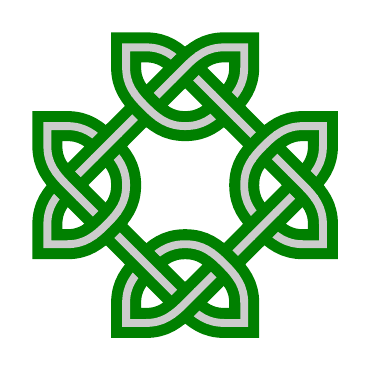
\begin{tikzpicture}[
  scale=.5,
  celtic path/.style={
    draw,
    double=gray!40,
    red,
    double distance=1mm,
    line width=4pt
  },
  celtic path 1/.style={
    green!50!black,
  },
]
\CelticDrawPath{
  symmetric crossings={
    1,2,-;
    2,1,|;
    4,3,-;
    3,4,|;
  },
  size={8,8},
}
\end{tikzpicture}
\end{center}

\section{Introduction}

This is a little TikZ library for drawing Celtic style knots.
The particular type of Celtic knot (technically, \emph{link}) is very simple and can be specified by listing the ``walls'' within the region of the knot.
From this information, it is possible to build the entire link and thus to tell TikZ how render it.
That is what this library does.

\section{Usage}

The routine is implemented as a TikZ library.
Thus to use it, add \Verb+celtic+ to the list of TikZ libraries that you load.

\begin{verbatim}
\usetikzlibrary{celtic}
\end{verbatim}

The library defines one command which renders a Celtic knot.
The knot is specified by passing various \emph{key-value} pairs to this command.
The library also defines styles which can be used to modify the rendering.

\DescribeMacro{\CelticDrawPath}\Verb+\CelticDrawPath{<opt>}+ is the command to render a knot.
It takes one option which is a list of key-value pairs which specify the knot.
The allowed key-value pairs are as follows.

\begin{itemize}
\item \Verb+max steps=N+ The process of finding the paths through the knot (needed to ensure that they are coloured correctly) is iterative.
Although every care has been taken to ensure that the iteration is confined (and therefore finite), the iteration has been devised with a built-in limit.
This limit can be adjusted using this key.
The default is \(20\).
If the limit is reached, a warning will be issued (and the knot will probably look wrong).
In that case, use this key to raise the limit.

\item \Verb+flip+ The specification of a Celtic knot in terms of walls does not completely determine it.
There is an ambiguity as to which crossings are over and which under (once one crossing is determined, all the others follow).
This key flips all of the crossings and so can be used to switch between the two variants.

\item \Verb+width=W+, \Verb+height=H+, \Verb+size={W,H}+ These set the dimensions on the knot in terms of the number of crossings.
The numbers must be even.

\item \Verb+crossings+, \Verb+symmetric crossings+ These set the crossings.
The general format of a crossing is \Verb+x,y,type+ where \Verb+x+ and \Verb+y+ can be either numbers or ranges, using the format \Verb+n:m+\footnote{This package uses \LaTeX3 internally; using a colon as the range separator was a headache to implement.}.
The type of the crossing is either \Verb+|+ or \Verb+-+ for (respectively) vertical or horizontal walls\footnote{The package attempts to be smart with regard to allowing \Verb+|+ to be active.}.
Multiple crossing specifications can be given as a semi-colon-delimited list (a final semi-colon is acceptable, making it easy to comment out items in the list).
The \Verb+symmetric+ variant places walls at four points obtained by applying reflections to the specified crossing.

\item \Verb+ignore crossings+, \Verb+ignore symmetric crossings+ The code works out the paths involved by picking a starting point and direction and then following it, bouncing off walls as appropriate, until it comes back to the beginning.
It then picks a new starting point and continues until all crossings are used up.
These keys designate certain points as \emph{disallowed} as starting points.
This can be used to remove certain regions from the knot, for example to create a border around a rectangle.
The \Verb+symmetric+ version works \dots\ symmetrically.

\item \Verb+style={<style>}+ The contents of this are passed on to \Verb+\tikzset+.
(The key-value pairs for the \Verb+\CelticDrawPath+ are actually \LaTeX3 keys, not TikZ keys, so this is the simplest way to pass them through.)

\item \Verb+at=<coordinate>+ This shifts the knot so that the lower left corner is at the coordinate.
(The default location is \Verb+(0,0)+.)
The coordinate is passed through TikZ's processing so can be any legal TikZ coordinate.

\item \Verb+inner clip=N+, \Verb+outer clip=N+.  The crossings are rendered by redrawing the over paths with a clipping region.
The size of the clipping region is determined by the line width.
These keys add a little to that clipping region.
This can be useful if the overdraws are not large enough, but the added amount should not be so much that the overdraws interfere with each other.
Some experimentation is needed.
The \Verb+inner clip+ applies to the background part of the path and the \Verb+outer clip+ to the foreground.

\end{itemize}

As the pieces are rendered, various TikZ styles are invoked.

\begin{itemize}
\item \Verb+celtic surround+ This style is used for the outer border.

\item \Verb+celtic bar+ This is used for the internal walls.
It is also used on the outer border (prior to the \Verb+celtic surround+ so it can be overridden).

\item \Verb+celtic path+ This is used for the components of the celtic knot (link).

\item \Verb+celtic path N+ The individual components can be styled using their number (there is a logic to the numbering, but experimentation is the best way to work out which is which).


\end{itemize}

\section{Example}

\begin{example}
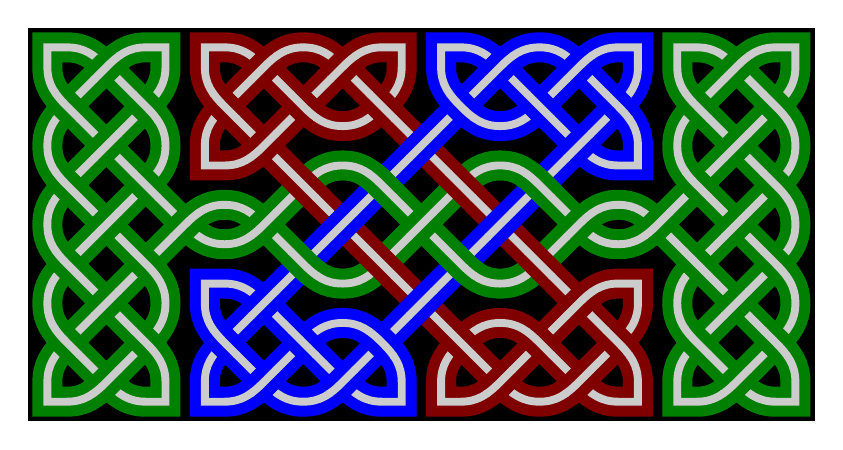
\begin{tikzpicture}[
  scale=.5,
  celtic path/.style={
    draw,
    double=gray!40,
    red,
    double distance=1mm,
    line width=4pt
  },
  celtic path 1/.style={
    green!50!black,
  },
  celtic path 2/.style={
    blue,
  },
  celtic path 3/.style={
    red!50!black,
  },
  celtic surround/.style={
    ultra thick,
    black,
    fill=black
  },
]
\CelticDrawPath{
  symmetric crossings={
    4,1:3,|;
    10,1,|;
    5,4,-;
    8,3,-;
  },
  size={20,10},
  max steps=50
}
\end{tikzpicture}
\end{example}

\begin{example}
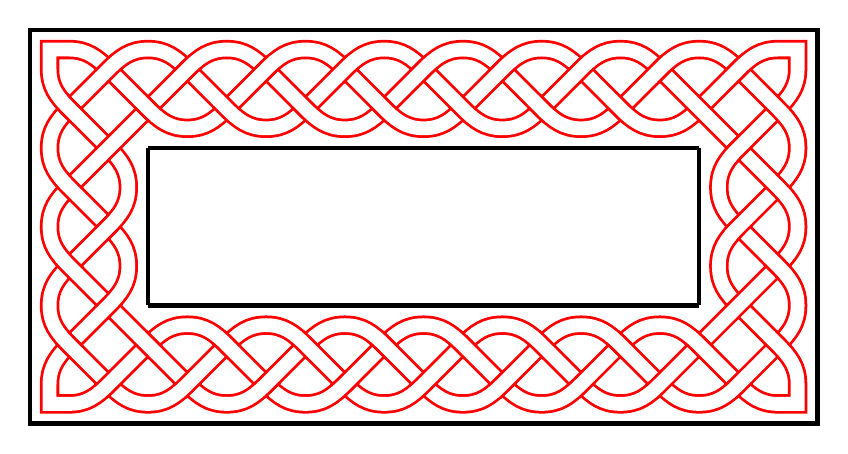
\begin{tikzpicture}[
  scale=.5,
  celtic path/.style={
    draw,
    double=white,
    red,
    double distance=5pt,
    line width=1pt
  },
  celtic bar/.style={
    ultra thick,
    black,
    draw
  },
]
\CelticDrawPath{
  size={20,10},
  symmetric crossings={
    3,4:5,|;
    4:16,3,-
  },
  ignore symmetric crossings={
    4:10,5;
    5:10,4
  },
  max steps=50
}
\end{tikzpicture}
\end{example}

\end{document}

% Local Variables:
% tex-output-type: "pdf18"
% End:
